\chapter{GLOBAL MOTOR INVARIANT}
\label{chap:gi}
\section{Introduction}

\nomenclature{$q$}{Generalized Coordinates}
\nomenclature{$Q$}{Configureation Space or Configuration Manifold}
\nomenclature{$\qd$}{Gneralized Velocity}
\nomenclature{$TQ$}{Tangenet Bundle of $Q$}
\nomenclature{$u$}{Control Input}
\nomenclature{$\state$}{State Variable}
\nomenclature{$M$}{State Space Manifold}
\nomenclature{$TM$}{Tangent Boundle Manifold}
\nomenclature{$A$}{Attractor}
\nomenclature{$B(A)$}{Basin of Attration of $A$}
\nomenclature{$S$}{Neural Oscilator}
\nomenclature{$\uin$}{Input Signal to the Neural Oscilator}
\nomenclature{$\uout$}{Output of the Neural Oscilator}
\nomenclature{$\hin$}{Input Coefficient of the Neural Oscilator}
\nomenclature{$\hout$}{Output Coefficent of the Neural Oscilator}
\nomenclature{$\simeq$}{Topology Conjungacy}


%\nomenclature[zcif]{$CIF$}{Cauchy's Integral Formula}                                % first letter Z is for Acronyms 
%\nomenclature[aF]{$F$}{complex function}                                                   % first letter A is for Roman symbols
%\nomenclature[gp]{$\pi$}{ $\simeq 3.14\ldots$}                                             % first letter G is for Greek Symbols
%\nomenclature[gi]{$\iota$}{unit imaginary number $\sqrt{-1}$}                      % first letter G is for Greek Symbols
%\nomenclature[gg]{$\gamma$}{a simply closed curve on a complex plane}  % first letter G is for Greek Symbols
%\nomenclature[xi]{$\oint_\gamma$}{integration around a curve $\gamma$} % first letter X is for Other Symbols
%\nomenclature[rj]{$j$}{superscript index}                                                       % first letter R is for superscripts
%\nomenclature[s0]{$0$}{subscript index}                                                        % first letter S is for subscripts



\ifpdf
    \graphicspath{{GlobalInvariant/GlobalInvariantFigs/PNG/}{GlobalInvariant/GlobalInvariantFigs/PDF/}{GlobalInvariant/GlobalInvariantFigs/}}
\else
    \graphicspath{{GlobalInvariant/GlobalInvariantFigs/EPS/}{GlobalInvariant/GlobalInvariantFigs/}}
\fi

Motion varies greatly, different people walk with different gait. 
A question is why the different motions of different people are all called walk.
Our answer is walk is not determined by the details how it is carried out.
Walk capture the qualitative properties, and we agree on the walk becomes it is a property encoded in all our body, we all have the walking ability inborn, so that’s the reason why we can all identify it.


Our basic idea is motion primitives are ''easy'' to finish. 
In this chapter, we will try to give the “easiness” definition.
The biological ideas can be provide a clear mathematical meaning.


\section{Basic Concepts of Qualitative Dynamics}
This section develops the mathematical conceptualization of Global Motor Invariant.
Some mathematical background is needed in this discussion.
Throughout this paper, we take the geometrical viewport of mechanical system.
For analyzing qualitative properties, we introduce the ideas from differential topology.
This idea can be traced back to Poincare\citep{Poincar'e1899,Poincar'e1885} and recently developed by the Smale School\citep{Smale1970}.
It is impossible to put the a whole discipline in one chapter.
Please refer to other books and lectures such as \citep{abraham1978foundations}for introduction in details.


Dynamic motions are modelled as differential equations,
In the geometrical viewport, differential equation describes a differentiable manifold.
Qualitative Properties can be obtained by analyzing the topological structure of the differentiable manifold.
Global Motor Invariant is defined by the topology structure.



\subsection{Dynamic System and Differential Manifold}



The dynamic of a mechanical system is determined by its configuration  $q$ and generalized speed $\qd$. 
we represent the state of a system as a vector $\state=[q,\qd] \in M$,  $M$ is the state space, or state manifold.
The motion is a trajectory $t \mapsto q(t)$ in the configuration space parameterized by time~$t$.
For a dynamic system, $q(t)$ usually is derived from the state trajectory $\state(t)$, which is described by differential equaiton. 


For every point $x \in M$, 
$F$ and $u$ determines a derivative vector $\dot{x} in T_{x}M$ in the Tangent Space. 
All the vectors over the full space of $x$ form the \textbf{vector field} $\mathbf{V}$,describe by the differential equaiton~ \ref{eq:ode}
which described by the differential equation
\begin{equation}
\label{eq:ode}
\dot{\state}=F_a(\state,u),\state\in M
\end{equation}

where $u$ is the control effort. 
$a$ is the system parameters
$F$ is determined by the system's natural property.
If $u=0$,  no control effort is applied.
Such systems are \textbf{autonomous systems}. 

By solving the \textbf{intergral curve}to equation~\ref{eq:ode}, 
\textbf{flow} $\Phi(\state)$ of $\mathbf{V}$ is the \textbf{intergral curve} through $\state$. 
all the flows form the \textbf{phase portrait}, which illustrates all the possible motions of the dynamic system.
We usually visualize the differential manifold by \textbf{phase plot}.


An illustrative example repeatedly used in this report is the mass-spring system. 
After linear transformation,  
a linear mass spring system can be described in canonical form equation ~\ref{eq:mass-spring}
where $q$ is the position of the mass, $\qd$ is the speed, and $\ddot{q}$ is the acceleration of mass.
 
If we chose the state variable $\state=[q,\qd]$, the ODE model should be in the form of equation~\ref{eq:stateform}
\begin{equation}
\label{eq:stateform}
\dot{\state}=
\left[ 
\begin{array}{cc}
0 &1\\
-1 &0 
\end{array}
\right]\state
\end{equation}



\subsection{Global Motor Invariant}
Flows can only intersect at some special position called \textbf{equilibria}.
Basically there are three type of equilibrium.
At each \textbf{equilbria}, 
the local space can be divided into three subspace of sub manifold: centre sub manifold, stable manifold, and unstable sub manifold.
\begin{description} 
\item[centre sub manifold]
If a flow $\phi$ pass through a point $\state_{c}$ on centre sub manifold $W_{c}$,
flow$\phi$ will remain on the Centre Manifold 
\[
\phi_{c}(t) \in W_{c}, t \in R
\]
 An equilibria must be on center manifold. 
\item [stable sub manifold]
For the flow $\phi_{s}$ passes through a point $\state_{s}$ on stable sub manifold $W_{s}$, the flow will finally converge to a no wandering point on centre sub manifold.
\[
\phi_{s}(+\infty)=\theta_{c}
\]
\item[unstable sub manifold]
For the flow $\phi_u$ passes through a point $\state_u$ on unstable sub manifold $W_{u}$, the flow will be repelled from the no wandering points on centre manifold.
An alternative perspective is the inverse of the flow converge to no wandering point. 
\[
\phi_{u}(-\infty)=\theta_{c}
\] 

\end{description}

The size and dimension of each sub manifold varies.
For some cases, the $W_{s}$ ( $W_{u}$) may not exist, 
this can be seen as the dimension of $W_{s}$($W_{u}$) is $0$.
\textbf{Attractors} are the equilbria where the whole local space is stable, the dimension of unstable submanifold is zero $\mathbf{dim}(W_{u})=0$.
\textbf{Repellors} are the equilibrias where the whole local space is unstable,the dimension of stable submanifold is zero $\mathbf{dim}(W_{s})=0$.







In theory, only observe the attractor of the dynamic system can be observed, motion task should be only rely on the attractor.
Two types of attrator are of great interest in motor control:(1) fixed point, as show inf Figure~\ref{fig:StablePosture},(2)Limit Cycle,as shown in Figure ~\ref{fig:limit_circle}

\begin{figure}
\begin{center}
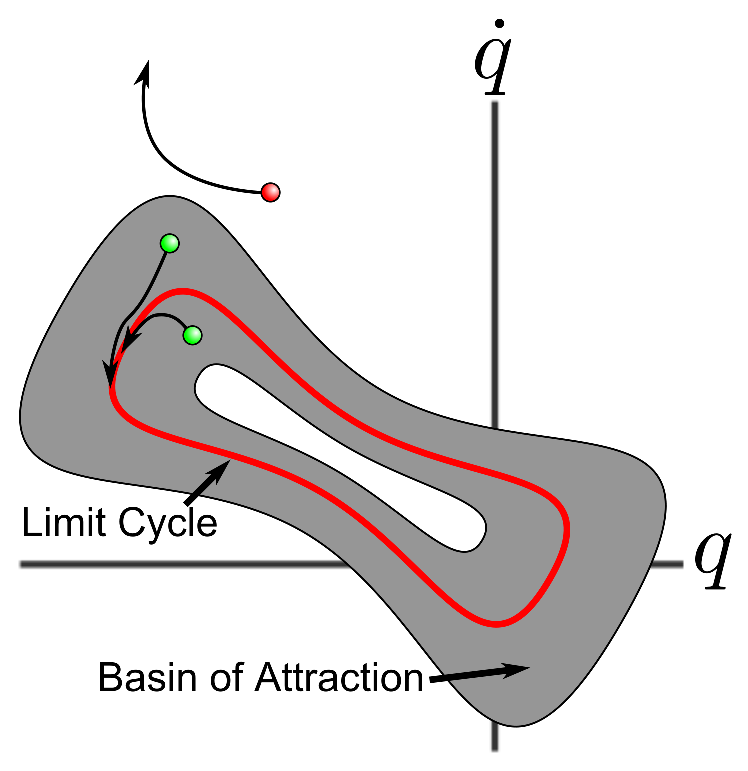
\includegraphics[height=0.4\textheight]{phase_plot}
\end{center}
\caption{Limit Cycle}
\label{fig:limit_circle}
\end{figure}




For nonlinear system, globally, the shape of stable and unstable sub manifold may be bending and connect with itself or each other.
The unstable manifold of one equilibrium may be the stable sub manifold of another.
The equilibra and its connectivity sub manifold form a topological structure.
Thus the phase plane will be divide into different regions,result in a cellular structure.
there is only one attractor, all the flow in this region will converge to the attractor ~$A$.
and the corresponding region is called basin of attraction ~$B(A)$.
as shown in figure~\ref{fig:manyboa}
\begin{figure}
\begin{center}
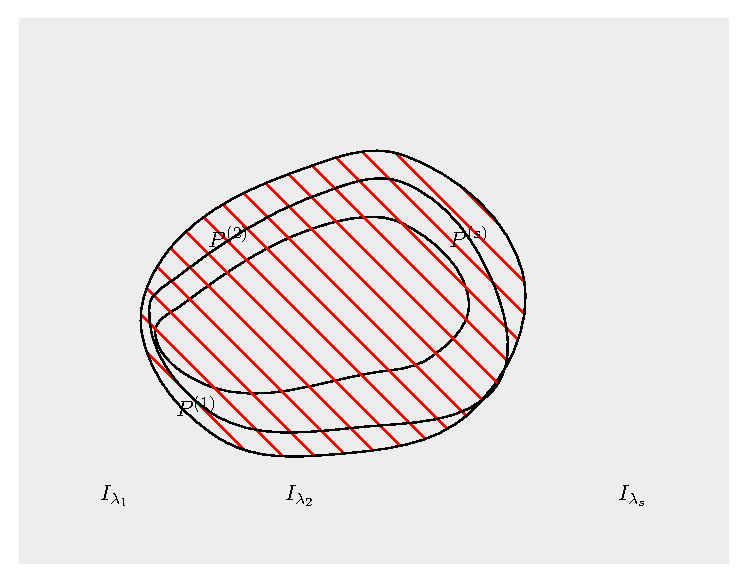
\includegraphics[height=0.4\textheight]{basinOfAttraction}
\end{center}
\caption{Celluar Structure of Phase Space}
\label{fig:manyboa}
\end{figure}


We can also give the biological ideas clear mathematical meaning.
The UMH, the uncontrolled manifold is the basin of attraction.
For EPH, the equilibrium point is the attractor.
For Impendence Control, impedance control is control the shape of basin of attraction.

\subsection{Analogous System And Topology Conjugacy}
many dynamic system are have different dynamic equation, but they share the same topology.
an example is the mass-spring system and the duffine system, described by equation ~\ref{eq:fuffin}
\begin{equation}
\label{eq:duffin}
\ddot{q}+q+q^{3}=0
\end{equation}
and the phase plot of the two system are show in figure~\ref{fig:msphaseplot},\ref{fig:duffin}

\begin{figure}
\begin{center}
\includegraphics[height=0.4\textheight]{massspring}
\end{center}
\caption{Mass Spring System}
\label{fig:msphaseplot}
\end{figure}

\begin{figure}
\begin{center}
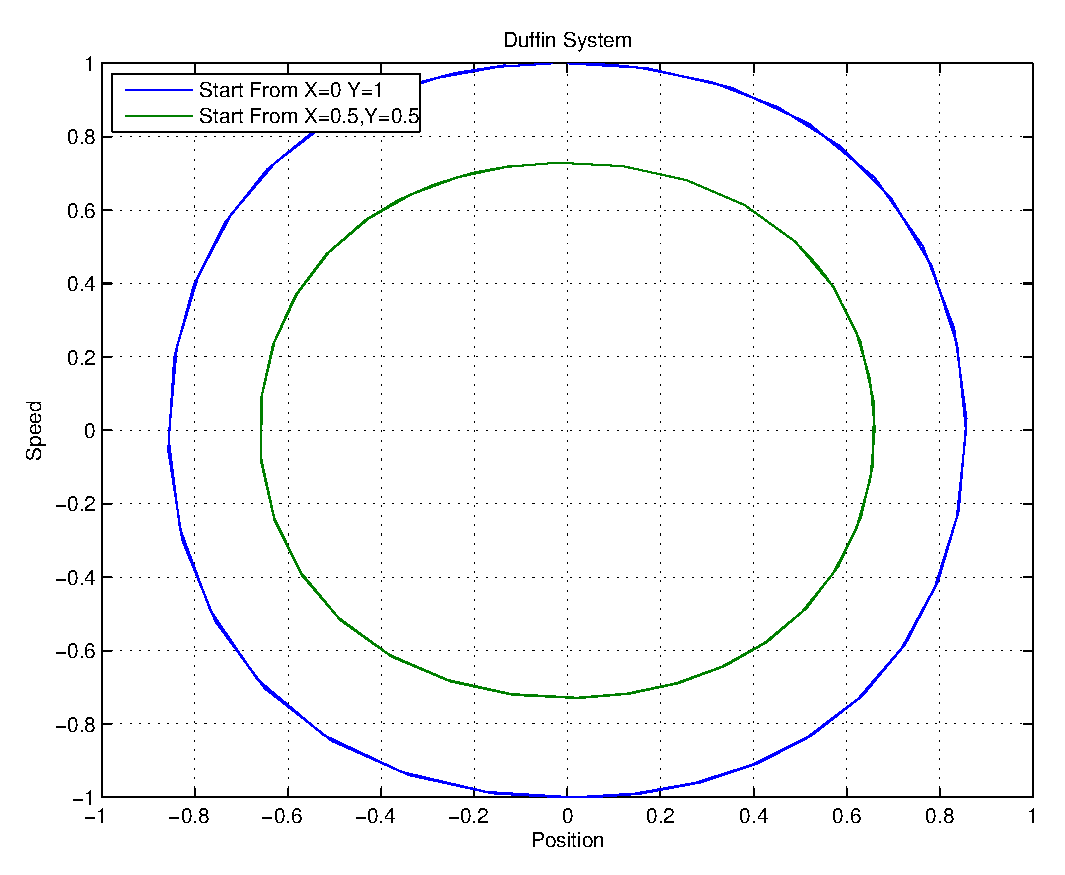
\includegraphics[height=0.4\textheight]{duffin}
\end{center}
\caption{Duffin Phase Plot}
\label{fig:duffin}
\end{figure}


one phase plot, the two system are similar, and we cand '' deform '' one into another.
in mathematical term, there is an equilalence relationship  for the two system. the \textbf{topological conjugacy}.

Let $X$ and $Y$ be topological spaces, and let $f\colon X\to X$ and $g\colon Y\to Y$
be continuous functions. We say that $f$ is
\emph{topologically semiconjugate} to $g$, if there exists a continuous
surjection $h\colon Y\to X$ such that $fh=hg$. If $h$ is a homeomorphism,
then we say that $f$ and $g$ are \emph{topologically conjugate}, and we call
$h$ a \emph{topological conjugation} between $f$ and $g$.



if two system are topological conjugate, they are analogous systems





\section{Global Motor Invariant and Motion Adaptation}
Global Motor Primitive is defined by the attractor type and its basin of attraction in the topology space.


Motion adaptation because of different reasons and in different situations.
Such two kinds of perturbation are treated separately and result in differentiation strategy or control.

\begin{itemize}
\HiItem{State perturbation}

The perturbation that move the state off the attractor is called State Perturbation, for only the state is changed, the dynamic system underline is not changed.


If the state is in the basin of attraction then, it will converge to the attractor. 
Start from different state position, it will result different flows, thus different motion.

Such kind of motion adaptation is called Responsive Motion Adaptation.
Because usually, for characters, perturbation comes from the push or pull, while the character and environment is not changed.

To make the character more responsive without result in motion failure,
Motion controller should try to enlarge the basin of attraction.






\HiItem{Structure Perturbation}

Another type of Perturbation will affect the dynamic system; such kind of perturbation is called Structure Perturbation. 
Such kind of perturbation happens commonly in our daily life, when a man put a heavy box on his shoulder, it will result a change in the dynamic system.

Structural Perturbation will change the phase portrait; some perturbation will make the system into an analogous system.
As a result, the even the current state is on the attractor, motion will change, this kind of motion adaptation is called system adaptation, and one important application is dynamic motion retargeting, when you change the character, the dynamic system changed.

Sometimes it will change the topology the underlying dynamic system, such effects are called bifurcation.
an example is the damping effects on the mass spring system.
as show in figure~\ref{fig:dampmass}

\begin{figure}
\begin{center}
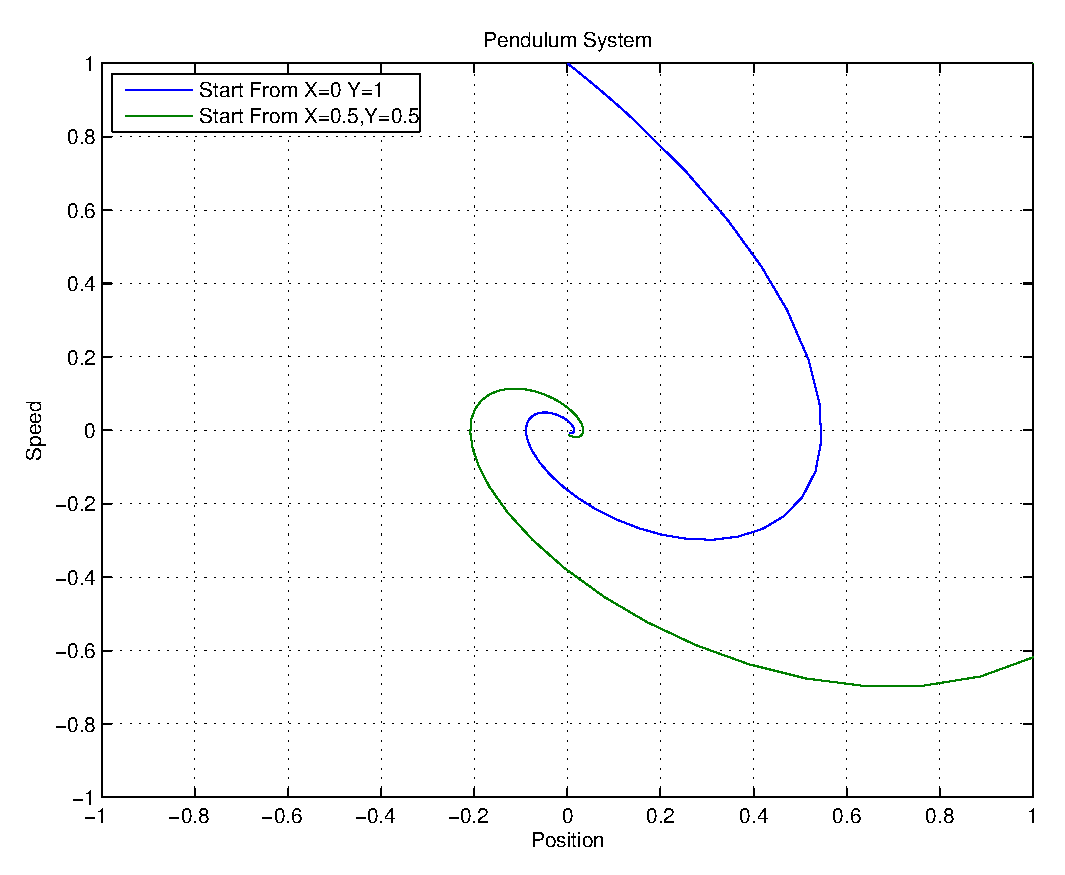
\includegraphics[height=0.4\textheight]{spring_damping}
\end{center}
\caption{damping perturbation onmass spring system}
\label{fig:dampmass}
\end{figure}

If ability of a dynamic system maintains its topology structure is structural stability.
To make characters more adaptive to environment and body change, motor controller should boost the structural stability of the motion.
Control effort should be prevent bifurcation.
\end{itemize}


\subsection{remarks on biological motor control}
Structural Stability is neglected in CMS research.
It is reasonable for natural animals to rely on structural stable autonomous system. 
In natural environment, perturbation and uncertainty are everywhere. In many cases, if neural system
can’t respond quickly enough, the better solution is to select a more structure stable motion primitives.

Structural Stability and Qualitative Idea provides a better explanation for some motion phenomena than quantitative theory like optimization and feedback shooting.
Qualitative Control Theory may help us understand the evolution of locomotion and neural Control.
Animals shift from the sea to the land. From quantitative computing viewport, the natural dynamics of the body and fluid environment are hard to predict or compute precisely. From the qualitative viewport, fluid is continuous
and uniform, the topology structure is very simple and stable, thus with little neural control fish can maintain its posture. On the other side, for human walking, although the rigid like
Environment can be calculated precisely, the topology structure is much more complex. 
Onthe phase plane, there exist many equilibrium points, the topology structure is more complex and unstable. 
The control system has to be more complex to control the more complex qualitative properties.

Qualitative theory can also help to explain another fact of biological motion system. 
Animals that live in similar environment and moves in a similar manner usually have similar body structure, in spite of their different position on evolution chain. 
This is because animals moving in a similar is based on the same motion primitive, similarity in body structure promise the topologial conjugacy.

This idea may help us to understand the body and environment effect in morphological computation theory. 
For specific environment, body evolves to provide us with a structural stable dynamic system, thus save lots of control effort for neural control.

We can also know motion primitives are not only defined by the body, it also defined by the environment, for motion in a specific environment, the topology should be fixed, thus the number of motion primitives is quite limited.


\section{Global Motor Invariant Control}
\subsection{CPG and Entrainment}
In nature, an animal's body and environment can be extremely complex. 
It leads to high dimensional manifolds with complicated topological structure, which provides many motion primitives for our use.
For CMS application, one question we want to ask is the so many motion primitives can be controlled with a simple method.

We propose that even there are many type of motion primitives, the type of attractor is limited. Basically there are only two types of attrator, limit circle and fix point.
Even the dimension of dynamic system maybe large, the dimension of the attrator is known. 
For fix point, its attractor is of dimension zero.
For limit circle, it is of dimension one.
Thus we can only focus on the type of attractor.



Biology Research suggested that the motor is mainly controlled by the Central Pattern Generator, which is a small autonomous network that generating rhythmic signals.
The idea of control motion by rhythmic signals can be modelled as entrainment \citep{Gonz'alez-Miranda2004}.
When coupling two oscillation system together, entrainment can happen when two system oscillator in synchronize. 
This effect will enhance the oscillation and also know as resonant. 




In previous section, we discussed two types of attractors: Fixed point and Limited Cycle. 
It is a still open question which type is more important and serve as the foundation as motor control\citep{Degallier2010}.
One idea limit circle is a necessary, fix point can be controlled with by 
(1) terminate a circle, 
(2)a different controller, 
(3)approximate by a limit circle with small amplitude or damping the limit circle, 
(4) change the limit circle into a fix point through by bifurcation. 



In this paper, 
\begin{itemize}
\HiItem Periodic behaviour is very common in biological systems. 
Besides the periodic motion in swimming and running, heart beating, wake and sleep also show periodic behaviour.
A periodic system has the potential to integrate with other bio system simulation to explore other motion features.

\HiItem Periodic motion has the same effect of terminated motion when the amplitude of limited circle is very small. 
For CMS research, both type of motion trajectory can be simulated with periodic motion.

\end{itemize}

\subsection{Neural Oscillator Stability}


Although it is difficult for neural system to carry out complex computation, it is easy to build oscillator structure with neurons. 
It only needs two neurons with mutual inhibitive property.
One extensively studied oscillation model is developed by \citet{neurooscillation}. 
The mathematical presentation is as follows:
\begin{eqnarray}
\tau_{1} \dot{s_{1}}&=&c-s_{1}-\beta l_{1}-\gamma [s_{2}]^{+}-\sum_{j}h_{j}[w_{j}]^{+}\\
\tau_{2} \dot{l_{1}}&=&[s_{1}]^{+}-l_{1}\\
\tau_{1} \dot{s_{2}}&=&c-s_{2}-\beta l_{2}-\gamma [s_{1}]^{-}-\sum_{j}h_{j}[w_{j}]^{-}\\
\tau_{2} \dot{l_{2}}&=&[s_{2}]^{+}-l_{2}\\
y_{i}&=&\mbox{max}(s_{i},0)\\
y_{o}&=&=[s_{1}]^{+}-[s_{2}]^{+}=y_{1}-y{2}
\label{eq:matsuta}
\end{eqnarray}

$c$,$\beta$,$\gamma$ are parameters of the oscillator,in our research are kept constant.
$\tau$ constrolls the oscilation frequency.







Matuoka oscillator is an autonomous oscillator; 
it can begin to oscillator without any control effort.
Figure ~\ref{fig:natural-oscilation} shows the natural oscillator output.
\begin{figure}[h]
\includegraphics[height=0.4\textheight]{oscillation.eps}
\caption{Natural Oscillation}
\label{fig:natural-oscilation}
\end{figure}





It is also adaptive; entrainment behaviour can happen between one Matuoka oscillator and different oscillators. 
Figure \ref{fig:entraint-oscilation} shows the entrain oscillation,
where the oscillation of Matuoka oscillator synchronise with the input signal.
\begin{figure}[h]
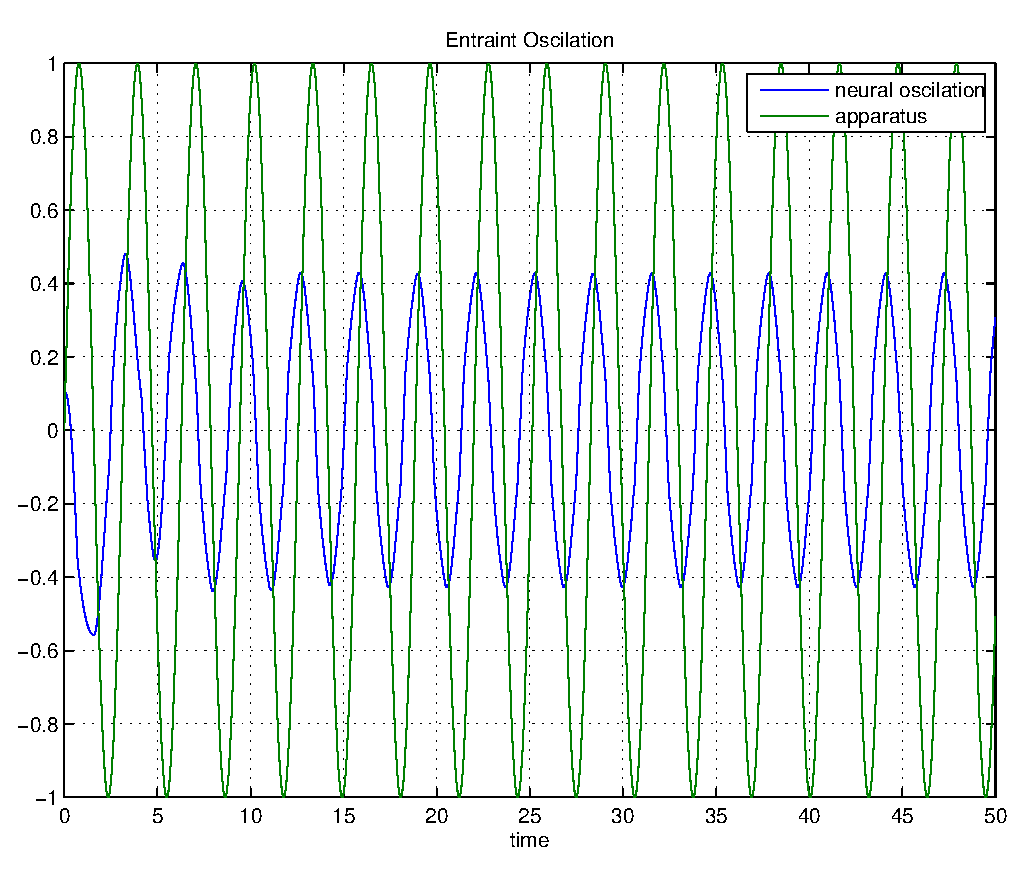
\includegraphics[height=0.4\textheight]{entraint_oscilation.eps}
\caption{Entrainment Oscillation}
\label{fig:entraint-oscilation}
\end{figure}

But because of the nonlinear properties, its behavior is not completely understood. 
Matsuta\citep{Matsuoka1987} explains the adaptive properties from the location of the roots of  characteristic equation. 
Wilimas\citep{Williamson1998} explains the properties in frequency domain.



In our research, we find some important properties of neural oscillator by empirical.

\begin{figure}
\begin{center}
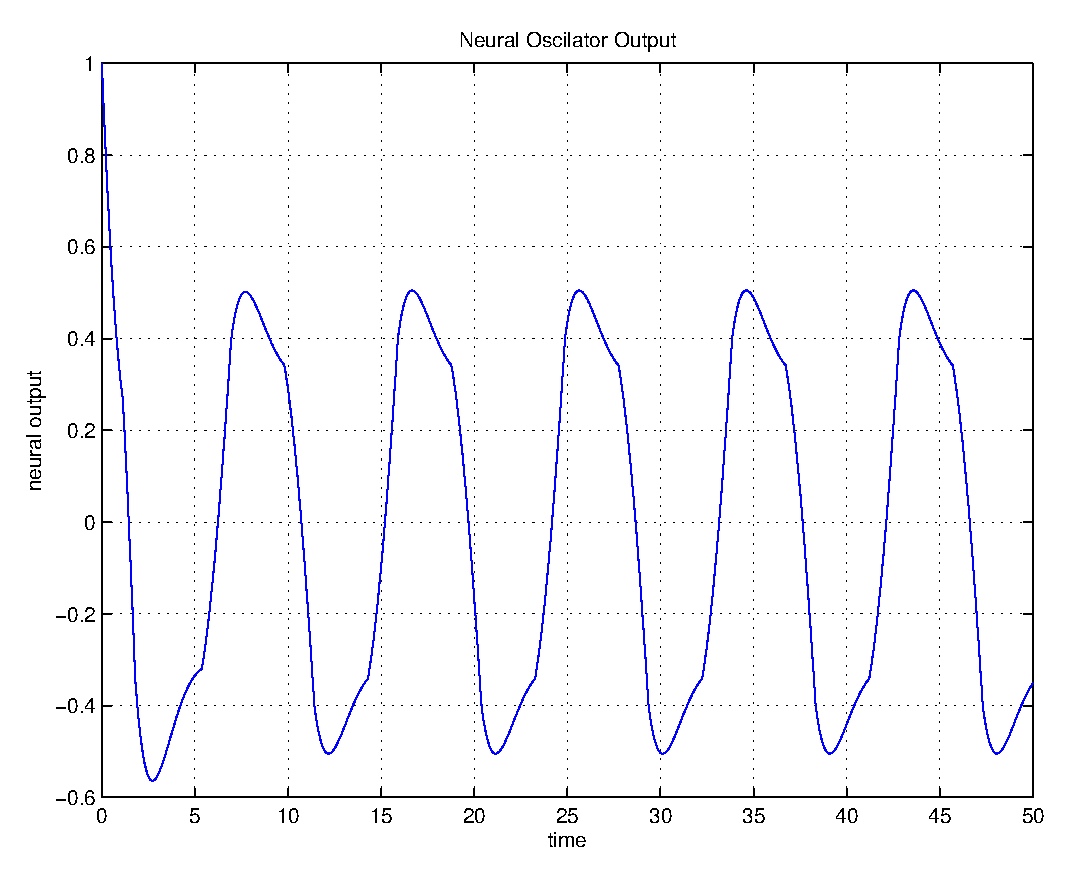
\includegraphics[height=0.5\textheight]{neuraloscilation1.eps}
\end{center}
\caption{The states of neural oscillator over Time}
\label{fig:oscilation}
\end{figure}

\begin{figure}
\begin{center}
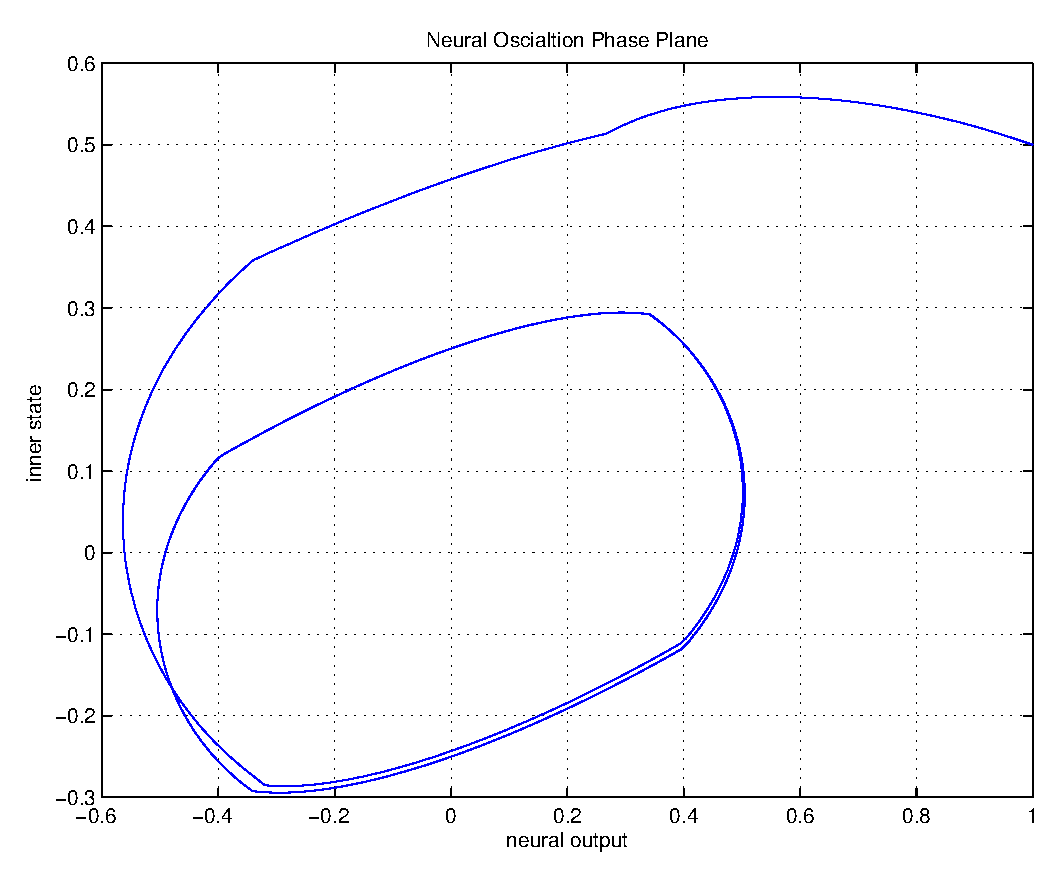
\includegraphics[height=0.5\textheight]{neural1phase.eps}
\end{center}
\caption{The phase portrait of Neural Oscillators}
\label{fig:oscilationphase}
\end{figure}

From our simulation, we investigate the topological structure.
Basically, neural oscillator shows three important properties:
\begin{itemize}
\item{Simple Topological Structure.}
The topology structure of neural oscillator is simple, 
it includes one  attractive limit circle and one fix repellor.
\item{Large Basin of Attraction.}
All the simulations we carried out converged to the same limited circle.
\item{Fast Converging Speed.}
In most of the case, the flow will converge to the limit circle within one period time.
\end{itemize}

Features above are shown in Figure ~\ref{fig:time_timeAttraction}.
\begin{figure}
\begin{center}
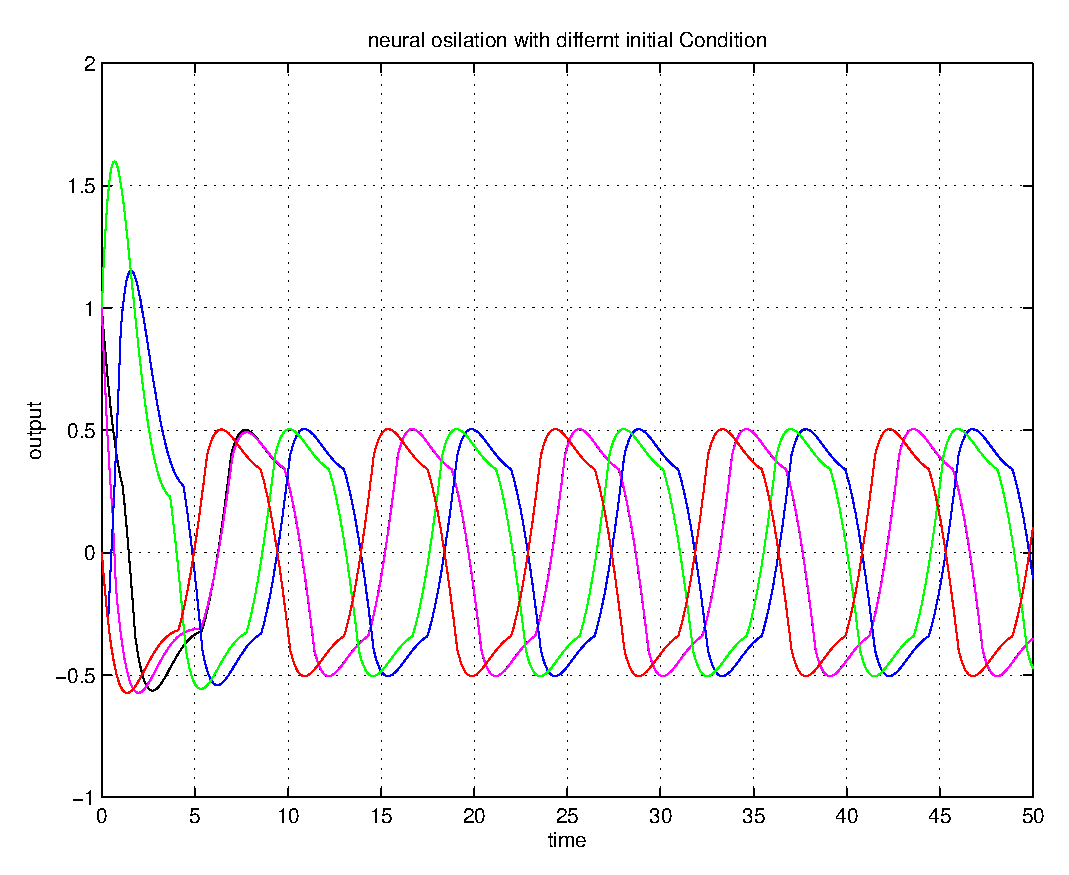
\includegraphics[height=0.4\textheight]{neural_attraction.eps}
\end{center}
\caption{Neural output with different initial position}
\label{fig:time_timeAttraction}
\end{figure}

\begin{figure}
\begin{center}
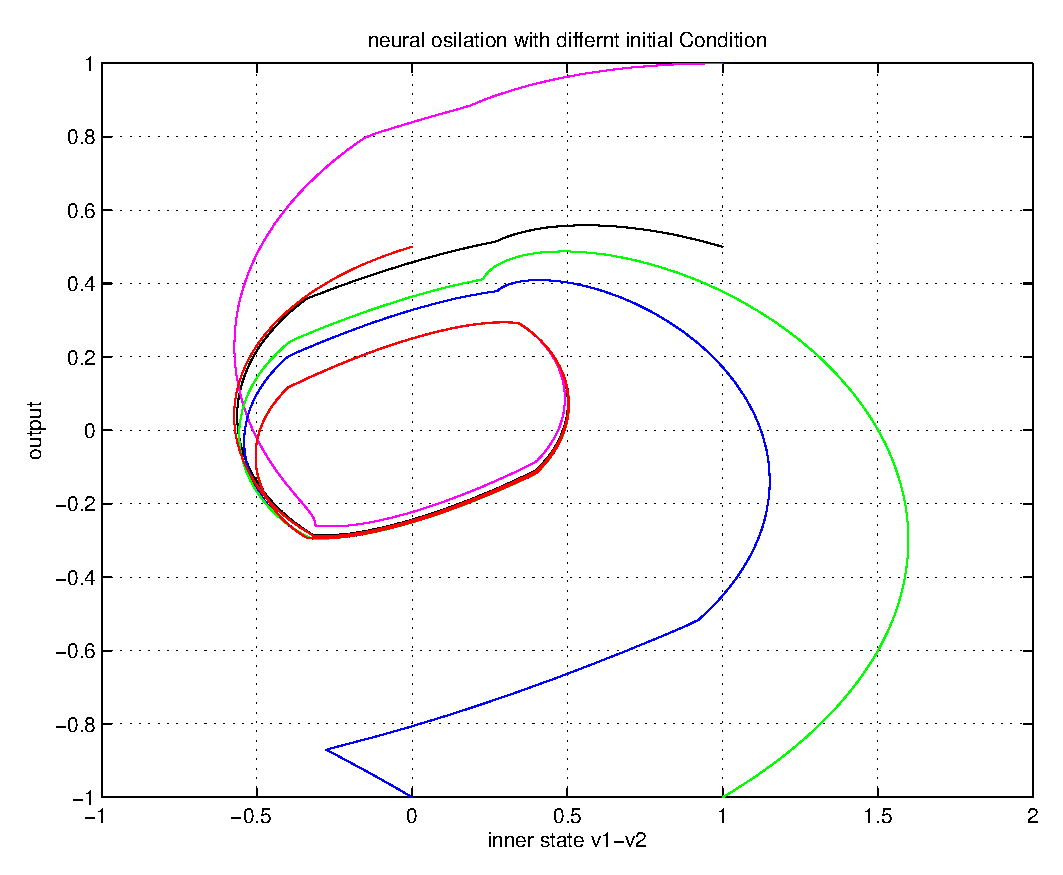
\includegraphics[height=0.4\textheight]{neural_attraction_phase.eps}
\end{center}
\caption{Phase plot of oscillation with different initial condition}
\label{fig:phase_attraction}
\end{figure}
 
The large area of basin of attraction means the final behaviour is totally determined by parameters. 
Initial condition will have no effects on the oscillator final output. 
Thus we treat matsuta oscilator as in a simple one input, one out put system, controlled by three parameter and input signal. 
we usually reformed equation ~\ref{eq:matsuta} in the simplified form
\begin{equation}
\label{eq:simplematsuta}
\uout=S_{[\hin,\hout,\tau]}(\uin)
\end{equation}
where $\uin=\sum_{j}h_{j}[w_{j}]=hw$,$\uout=\hout y_{o}$





The converging speed can be seen as quick recovery ability.
When an impulse perturbation happens, it will recover in one period time.


\section{Example:Maintain Bouncing Height}

Bouncing ball is system ball bouncing by moving a pedal, a system with simple dynamic but difficult to control with optimizaiton or pd. 
While this example capture the complexity of human interatction with the environment and object. 
And can be the basic model for many motion tasks.

We show in this example how neural oscillator can turn the bouncing ball system into motion primitive.
\subsection*{Dynamics}
Hybrid dynamics, in incoperate two phase, 
 

\begin{align}
\ddot{q}&=-g&\mathrm{if}\,\,q &> 0\,\,\mathrm{(free\,\,flying)} \nonumber\\
\dot{q}^{+}_{\mathrm{ball}} - \dot{q}^{+}_{\mathrm{paddle}} &=  \epsilon(\dot{q}^{-}_{\mathrm{ball}} - \dot{q}^{-}_{\mathrm{paddle}})&\mathrm{if}\,\,q &\leq 0\,\,\mathrm{(paddle\,\,strike)}\nonumber
\end{align}

Basically, the ball will continue bouncing with smaller height,as show in Figure~\ref{fig:bborg}.

\begin{figure}[h]
\begin{center}
	\subfigure[state plot]
	{
	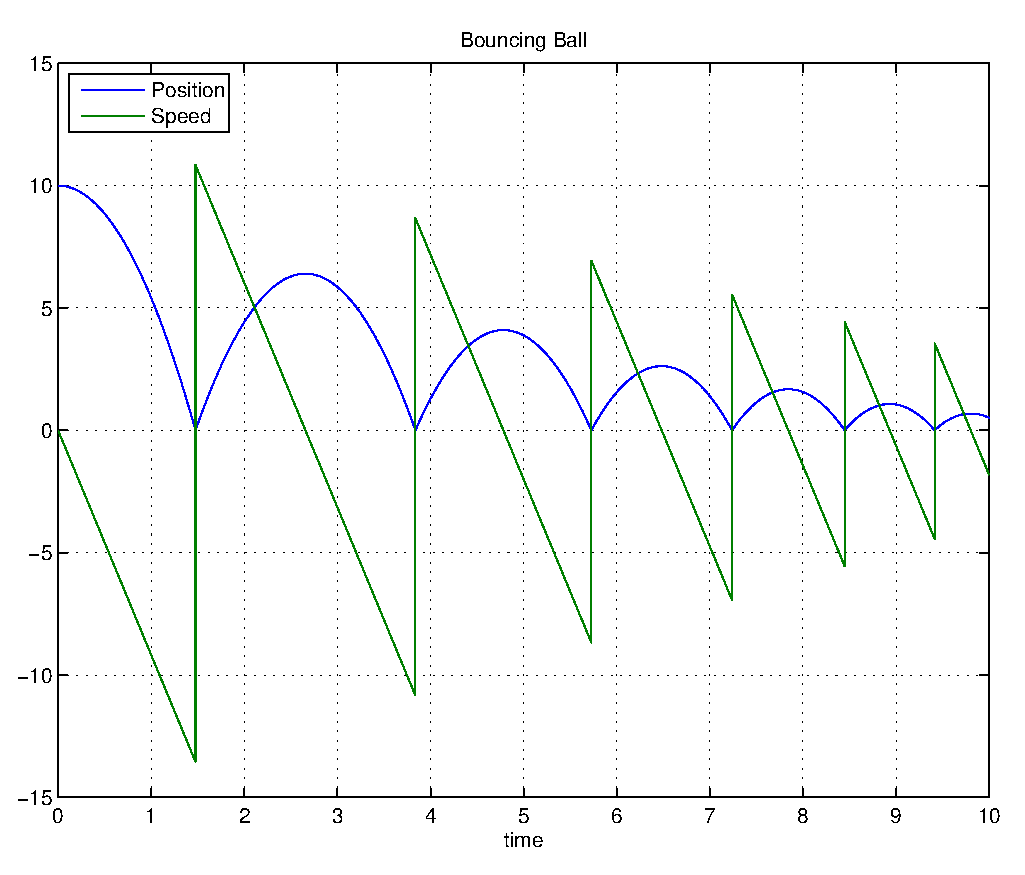
\includegraphics[width=0.45\textwidth]{bouncing_ball}
	\label{fig:bb}
	}
	\subfigure[Phase Plane]
	{
	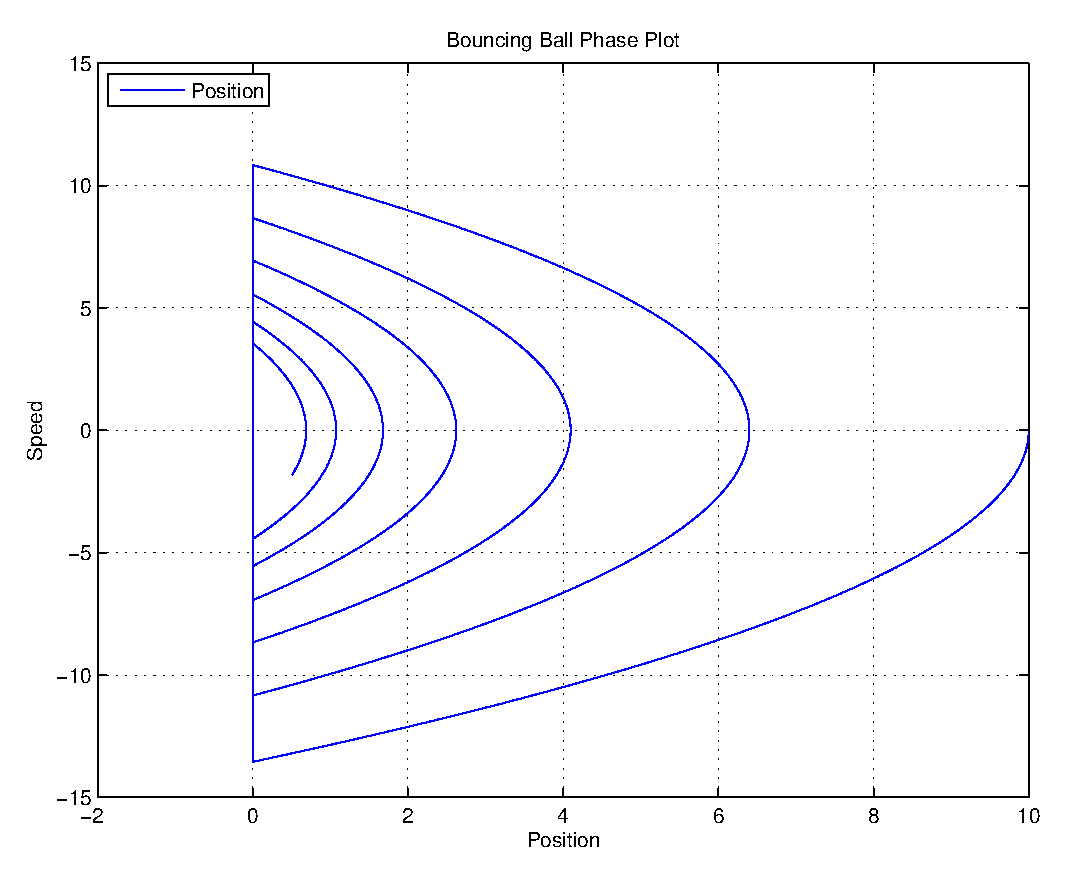
\includegraphics[width=0.45\textwidth]{bouncing_ball_phaseplot}
	\label{fig:bbp}
	}
	
\end{center}
\caption{Original Bourncing Ball System}
\label{fig:bborg}
\end{figure}



\subsection*{Emergence of Limit Cycle}
couple with neural oscillator boucing we get an limit circle
The input of neural oscillator is the velocity $\uin=\dot{q}_{ball}$, the output of neural oscillator  drive the pedal position $q_{pedal}=\uout$.
An limit circle emerge as the result of entrainment.
As show in figure drop from different position, all the ball will bouncing a about the same height of 5,as show in Figure~\ref{fig:bb_attractive_circle}

\begin{figure}[h]
\begin{center}
	\subfigure[state plot]
	{
	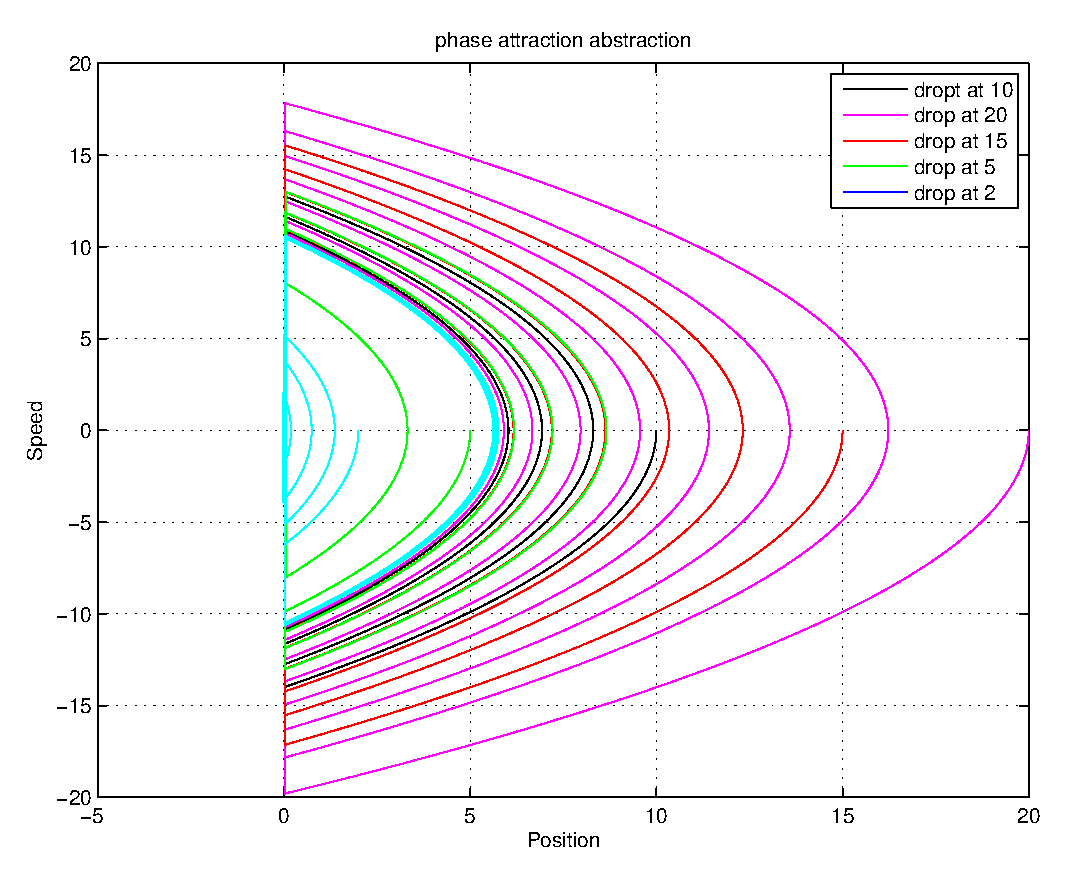
\includegraphics[width=0.45\textwidth]{bb_ms_os_attraction_phase}
	\label{fig:bb_attractive_entraint}
	}
	\subfigure[Phase Plane]
	{
	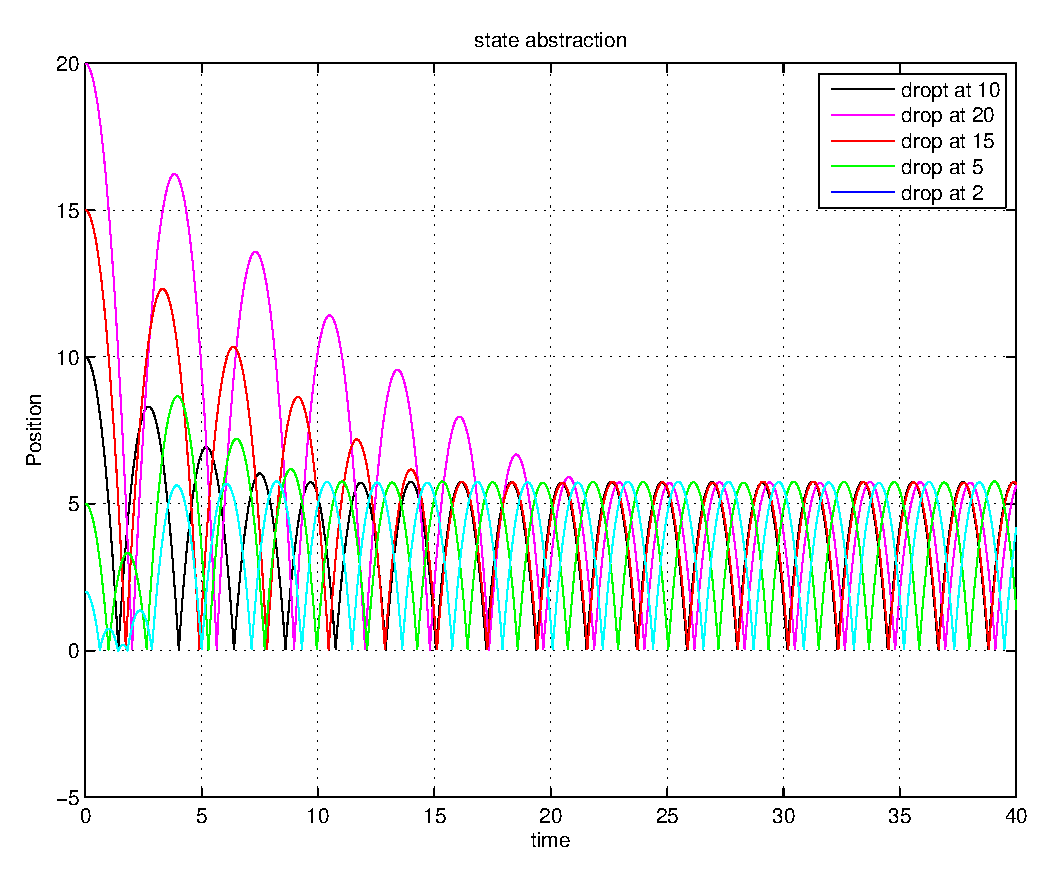
\includegraphics[width=0.45\textwidth]{bb_ms_os_StateTimeAttraction}
	\label{fig:bb_attractive_entraint_time}
	}
	
\end{center}
\caption{Attractive Limited Circle}
\label{fig:bb_attractive_circle}
\end{figure}
